\chapter{The International Linear Collider}
\label{ILC}
The International Linear Collider (ILC) is a linear \electron \positron accelerator with an center-of-mass energy of \unit{500}{GeV} in the first stage and \unit{1}{TeV} in the second.
The state of the art technologies for both, the detectors and the machine, and the machine design make a clean environment and high precision measurements possible, because of which the ILC will be a unique machine.\\
The following sections will talk about the ILC layout, its possible sites, the two detectors, and finally the physics motivation for such a capable accelerator.
\section{Layout}
\label{ILC:layout}

Figure~\ref{fig:ILC_Layout} shows the schmeatic layout of the ILC for the \unit{500}{GeV} stage.
The electrons originate in the polarised source based on a photocathode DC gun.
When these electrons pass through an undulator, high-energy photons are produced which are then converted to electron-positron pairs.
This is the polarised positron source.
The main linacs are extendable for the machine upgrade to \unit{1}{TeV}.

\begin{figure}
\centering
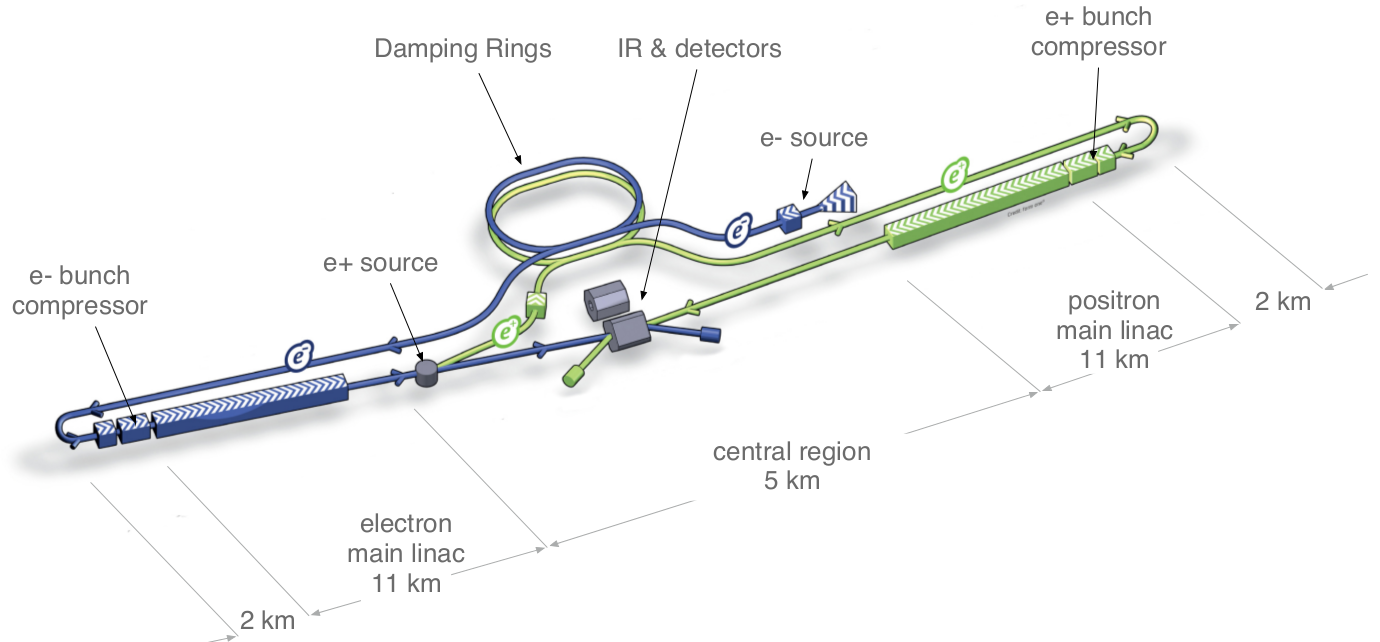
\includegraphics[width=0.8\textwidth]{Figures/ILC_layout.png}
\caption[Schematic layout of the ILC]{Schematic layout of the ILC~\cite[p. 9]{ILC1}}
\label{fig:ILC_Layout}
\end{figure}


\section{Possible Site}
\label{ILC:site}
\section{SiD and ILD}
\label{ILC:detectors}
\section{Physics Motivation}
\label{ILC:physicsmotivation}
